\section{DOM}

El \textbf{Modelo de Objetos de Documento} (\textbf{Documento Object Model}, abreviado DOM) es un modelo que contiene todos los objetos o estructura lógica de una página o sitio web.

Cuando el buscador busca acceder a un sitio web, primero carga toda la parte HTML de la misma para poder presentarlo en la pantalla, para lograr esto, construye el DOM del sitio, el cual puede ser representado o visualizado mejor en la \textit{Figura \ref{fig: 5}}:
\begin{figure}[H]
    \caption{Ejemplificación del DOM de HTML de un sitio web}
    \label{fig: 5}
    \begin{center}
        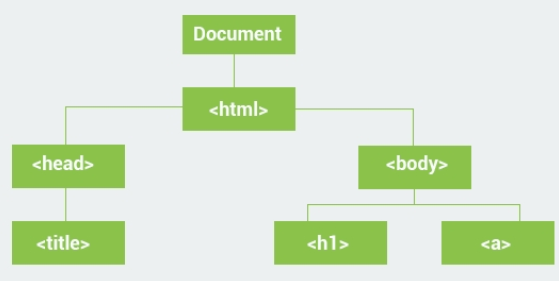
\includegraphics [width=9cm]{ss/dom_html.png}
    \end{center}
\end{figure}

Si refrescamos memoria, HTML se maneja por medio de etiquetas, una de apertura y una de cierre, dentro de las etiquetas podemos meter más etiquetas que cumplen con distintas funciones, lo que representa el DOM es esa jerarquía o árbol de etiquetas (ahora llamados \textbf{nodos}) que constituye un sitio web, que es lo que se ve en la imagen anterior (nodo raíz, hermanos, hijos, etc). En la previa imagen, tenemos que:
\begin{itemize}
    \item El nodo $<$html$>$ tiene dos hijos: $<$head$>$ y $<$body$>$.
    \item El nodo$<$head$>$ tiene un hijo: $<$title$>$.
    \item El nodo $<$title$>$ tiene un padre: $<$head$>$.
    \item El nodo $<$body$>$ tiene dos hijos: $<$h1$>$ y $<$a$>$.
    \item Los nodos $<$h1$>$ y $<$a$>$ tienen un padre: $<$body$>$:
    \item Los nodos $<$head$>$ y $<$body$>$ son hermanos o están al mismo nivel.
\end{itemize}

\textbf{JavaScript puede manipular el DOM de un sitio web} para volverlo dinámico y agregar, modificar o eliminar los nodos del DOM. Vimos al inicio de este documento que una de las formas de mostrar texto en un sitio web utilizando este lenguaje es por medio de \textbf{document.write()}, \textit{document} es un objeto de DOM disponible en JavaScript que te permite acceder los nodos del DOM, este objeto es el dueño (raíz) del resto de elementos de un sitio web.

Podemos ver representado lo anterior con el diagrama de la \textit{Figura \ref{fig: 6}}:
\begin{figure}[H]
    \caption{Visualización del DOM y su relación con JavaScript}
    \label{fig: 6}
    \begin{center}
        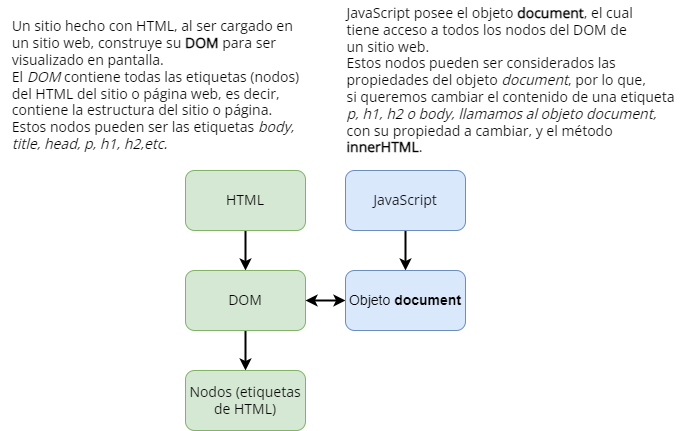
\includegraphics [width=13cm]{ss/dom_explicacion.png}
    \end{center}
\end{figure}

Presentamos también ejemplos de como se ve el uso del objeto \textbf{document} con las propiedades y métodos que posee:
\begin{lstlisting}
    // Declara variable que cambia el contenido de la etiqueta BODY.
    var cuerpo = document.body.innerHTML = "nuevo texto";
    // Declara variable que cambia el contenido de la etiqueta P.
    var parrafos = document.p.innerHTML = "NUEVO PARRAFO";
\end{lstlisting}

Basta con escribir el operador punto (.), seguido del nodo o etiqueta que queremos seleccionar, otro operador punto, y el método que queramos aplicar a la propiedad. \textbf{innerHTML()} es un método del objeto muy común de utilizar, cambia o devuelve el contenido de un nodo.


\subsection{Seleccionando elementos}

Entonces, \textbf{document} es un objeto que posee métodos y propiedades para interactuar con las propiedades de un sitio HTML, los siguientes métodos son los más utilizados para seleccionar elementos HTML:
\begin{lstlisting}
    // Encuentra un elemento por su ID.
    document.getElementById(id);
    // Encuentra un elemento por su nombre de etiqueta.
    document.getElementByClassName(nombre);
    // Encuentra un elemento por su etiqueta.
    document.getElementByTagName(etiqueta);
\end{lstlisting}

Volviendo a recordar HTML, sabemos que a una etiqueta podemos asignarle una clase o identificador, es por ello que los métodos anteriores buscan obtener uno o varios elementos a partir de la etiqueta que los representa, su identificador particular o clase:
\begin{lstlisting}
    <html>
        <head>
            <title>Prueba</title>
        </head>
        <body>
            <!-- Etiqueta con identificador -->
            <h1 id="cabecera">Hola mundo</h1>
            <!-- Etiqueta con clase asignada -->
            <p class="parrafos">Esto es un párrafo</p>
        </body>
    </html>
\end{lstlisting}

Por lo que, si utilizamos el método \textbf{getElementById()} o \textbf{getElementByClassName()} junto con \textbf{innerHTML}, podemos cambiar el contenido de las etiquetas con dicha clase e identificador:
\begin{lstlisting}
    <html>
        <head>
            <title>Prueba</title>
        </head>
        <body>
            <!-- Etiqueta con identificador -->
            <h1 id="cabecera">Hola mundo</h1>
            <!-- Etiqueta con clase asignada -->
            <p class="parrafos">Esto es un párrafo</p>
            
            <script>
                // Encuentra un elemento por su ID.
                var ej1 = document.getElementById("cabecera");
                ej1.innerHTML = "Hola mundo, nuevo texto.";
                // Encuentra un elemento por su nombre de etiqueta.
                var ej2 = document.getElementByClassName("parrafo");
                ej2[0].innerHTML = "Esto es un nuevo párrafo.";
            </script>
        </body>
    </html>
\end{lstlisting}

\textbf{getElementById} regresa únicamente un valor o elemento, ya que un identificador tiene la naturaleza de representar la identidad de un único elemento; \textbf{getElementByClassName} regresa una colección de datos (\textbf{un arreglo}), ya que múltiples etiquetas pueden estar modificados por una sola clase o varias, es por tal motivo que el código anterior tiene el operador llaves cuadradas con un índice.

\textbf{getElementByTagName} regresa también un arreglo con todos los elementos que tengan una etiqueta particular:
\begin{lstlisting}
    <html>
        <head>
            <title>Prueba</title>
        </head>
        <body>
            <p>hi</p>
            <p>hello</p>
            <p>hi</p>
            
            <script>
                // Encuentra un elemento por su etiqueta (p).
                var arr = document.getElementsByTagName("p");
                // Cambia el contenido de todos los elementos con etiqueta p.
                for (var x = 0; x < arr.length; x++) {
                    arr[x].innerHTML = "Hi there";
                }
            </script>
        </body>
    </html>

    /* Imprime:
    hi
    hello
    hi
    hi there
    hi there
    hi there
    */
\end{lstlisting}

La \textit{Tabla \ref{tab: 9}} contiene los métodos de los nodos para conocer su relación con otros nodos dentro del DOM:
\begin{table}[H]
    \begin{center}
        \caption{Métodos de nodos del objeto \textit{document}}
        \label{tab: 9}
        \begin{tabular}{c l}
            \hline
            \textbf{Método}&\textbf{Definición} \\
            \hline
            nodo.\textbf{childNodes}        & Regresa un arreglo con los nodos hijos del nodo \\
            nodo.\textbf{firstChild}        & Regresa el primer nodo hijo de un nodo \\
            nodo.\textbf{lastChild}         & Regresa el último nodo hijo de un nodo \\
            nodo.\textbf{hasChildNodes}     & Regresa true o false sin un nodo tiene hijos o no \\
            nodo.\textbf{nextSibling}       & Regresa el siguiente nodo del nodo actual en el mismo nivel \\
            nodo.\textbf{previosSibling}    & Regresa el nodo anterior del nodo actual en el mismo nivel \\
            nodo.\textbf{parentNode}        & Regresa el nodo padre del nodo actual \\
            \hline
        \end{tabular}
    \end{center}
\end{table}


\subsection{Cambiando elementos}

Ya vimos que con \textbf{innerHTML} podemos acceder o modificar el contenido de un nodo, ahora veremos que también podemos modificar las propiedades o atributos de los nodos:
\begin{lstlisting}
    <html>
        <head>
            <title>Prueba</title>
        </head>
        <body>
            <!-- Inserta una imagen y enlace -->
            <img id="mimg" src="banana.png"/>
            <a href="https://www.google.com">Esto es un enlace</a>
            
            <script>
                // Recibe el nodo con identificador "mimg".
                var el = document.getElementById("mimg");
                // Recibe arreglo con los nodos con etiqueta "a".
                var en = document.getElementByTagName("a");
                // Cambia la imagen y enlace de los respectivos nodos.
                el.src = "apple.png";
                en[0].href = "https://www.youtube.com";
            </script>
        </body>
    </html>
\end{lstlisting}

El estilo en cómo es presentado un nodo también se puede cambiar con JavaScript (color, fondo, alto, ancho, animación, etc). Todas las propiedades del lenguaje CSS pueden ser modificadas también con JavaScript, solamente recuerde que estas propiedades suelen utilizar mucho el guión (-) en sus nombres, por lo que, si desea cambiar una propiedad CSS con JavaScript, cree variables con el nombre de la propiedad, pero omitiendo el guión, dejando únicamente el nombre de la propiedad con mayúsculas y todo junto.
\begin{center}
    \textit{CSS: background-color\\JavaScript: backgroundColor}
\end{center}


\subsection{Agregando elementos}

Los métodos que aparecen en la \textit{Tabla \ref{tab: 10}} nos ayudarán a crear o eliminar nuevos y existentes nodos:
\begin{table}[H]
    \begin{center}
        \caption{Métodos para trabajar con nodos de \textit{document}}
        \label{tab: 10}
        \begin{tabular}{m{7cm} m{7cm}}
            \hline
            \textbf{Método} & \textbf{Definición} \\
            \hline
            nodo.\textbf{cloneNode()}                           & Clona un nodo \\
            document.\textbf{createElement(nodo)}               & Crea un nodo \\
            document.\textbf{createTextNode(texto)}             & Crea un nodo de solo texto \\
            nodo.\textbf{appendChild(nuevo nodo)}               & Agrega a un nodo otro nodo como último hijo \\
            nodo.\textbf{insertBefore(nodo1, nodo2)}            & Agrega a un nodo otro nodo1 hijo antes de otro nodo2 hijo \\
            nodo.\textbf{removeChild(nodo)}                     & Elimina un nodo hijo de un nodo padre \\
            nodo.\textbf{parentNode}                            & Regresa el nodo padre de un nodo \\
            nodo.\textbf{replaceChild(nodo1, nodo2)}    & Cambia un nodo por otro \\
            \hline
        \end{tabular}
    \end{center}    
\end{table}

Para los métodos que crean nodos, estos son creados pero no son adjuntados al DOM, por lo que deberán utilizar \textbf{appendChild()} o \textbf{insertBefore()} para poder adjuntarlos a la estructura HTML del sitio web:
\begin{lstlisting}
    <html>
        <head>
            <title>Prueba</title>
        </head>
        <body>
            <div id="prueba">Un texto</div>
            
            <script>
                // Crea un nuevo nodo "p".
                var p = document.createElement("p");
                // Crea un nodo solo de texto.
                var txt = document.createTextNode("Some new text");
                // Agrega el nodo solo texto al nodo "p".
                p.appendChild(node);
                // Recibe el nodo con identificador "prueba".
                var div = document.getElementById("prueba");
                // Agrega el nodo "p" al nodo con identificador "prueba".
                div.appendChild(p);
            </script>
        </body>
    </html>
\end{lstlisting}


\subsection{Eliminando elementos}

Si deseas eliminar un nodo del DOM, primero debes acceder a su nodo padre, utilizar el método \textbf{removeChild()}:
\begin{lstlisting}
    <html>
        <head>
            <title>Prueba</title>
        </head>
        <body>
            <!-- Crea un contenedor con identificador "demo" -->
            <div id="demo">
                <!-- Crea dos párrafos con identificador "p1" y "p2" -->
                <p id="p1">This is a paragraph.</p>
                <p id="p2">This is another paragraph.</p>
            </div>
            
            <script>
                // Recibe el nodo con identificador "demo".
                var padre = document.getElementById("demo");
                // Recibe el nodo con identificador "p1".
                var hijo = document.getElementById("p1");
                // Del nodo "padre" se elimina su nodo "hijo"
                padre.removeChild(hijo);
            </script>
        </body>
    </html>
\end{lstlisting}

En el ejemplo anterior, se elimina uno de los párrafos del contenedor div "demo". Podemos hacer esto de forma más directa con la propiedad \textbf{parentNode}:
\begin{lstlisting}
    padre.parentNode.removeChild(hijo);
\end{lstlisting}


\subsection{Reemplazando elementos}

Si requerimos quitar un nodo del DOM y poner otro para sustituirlo, podemos utilizar el método \textbf{replaceChild()}:
\begin{lstlisting}
    <html>
        <head>
            <title>Prueba</title>
        </head>
        <body>
            <!-- Crea un contenedor con identificador "demo" -->
            <div id="demo">
                <!-- Crea dos párrafos con identificador "p1" y "p2" -->
                <p id="p1">This is a paragraph.</p>
                <p id="p2">This is another paragraph.</p>
            </div>
            
            <script>
                // Crea un nuevo nodo "p".
                var p = document.createElement("p");
                // Crea un nodo solo texto.
                var nodo = document.createTextNode("This is new");
                // Asigna al nodo creado "p" el nodo solo texto ("p" con texto "This is new").
                p.appendChild(nodo);
                // Recibe el nodo con identificador "demo".
                var padre = document.getElementById("demo");
                // Recibe el nodo con identificador "p1".
                var hijo = document.getElementById("p1");
                // Remplaza el nodo hijo con el nuevo nodo "p".
                padre.replaceChild(p, hijo);
            </script>
        </body>
    </html>
\end{lstlisting}

Utiliza el mismo funcionamiento que el método anterior, donde primero debes seleccionar el nodo padre del nodo a reemplazar.



\section{Eventos}

Se puede ejecutar un bloque de código JavaScript cuando algo ocurre en el sitio web: un clic, el puntero encima de una etiqueta, recarga de la página, etc; a esto se le llama \textbf{evento}. La \textit{Tabla \ref{tab: 11}} contiene algunos de los eventos más comunes:
\begin{table}[H]
    \begin{center}
        \caption{Métodos para ejecutar eventos}
        \label{tab: 11}
        \begin{tabular}{m{3cm} m{10cm}}
            \hline
            \textbf{Evento} & \textbf{Definición} \\
            \hline
            onclick         & Ocurre cuando se da clic a un elemento \\
            onload          & Ocurre cuando un objeto ha sido cargado \\
            onunload        & Ocurre cuando una página no ha sido cargada (para $<$body$>$) \\
            windows.onload  & Realiza lo mismo que el evento onload \\
            onchange        & Ocurre cuando el contenido de un elemento de un \textit{form} ha cambiado (para $<$input$>$, $<$keygen$>$, $<$select$>$ y $<$textarea$>$) \\
            onmouseover     & Ocurre cuando el puntero está encima de un elemento o un hijo de este \\
            onmouseout      & Ocurre cuando el puntero sale de encima de un elemento o un hijo de este \\
            onmousedown     & Ocurre cuando el usuario presiona un botón del ratón encima de un elemento \\
            onmouseup       & Ocurre cuando el usuario deja de presionar un botón del ratón encima de un elemento \\
            onblur          & Ocurre cuando un elemento pierde el \textit{focus} \\
            onfocus         & Ocurre cuando un elemento obtiene el \textit{focus} \\
            onsubmit        & Ocurre cuando se envía un formulario \\
            \hline
        \end{tabular}
    \end{center}    
\end{table}


\subsection{Manejando eventos}

Los eventos son funciones de JavaScript, por lo que se los podemos asignar o adjuntar a una etiqueta en particular:
\begin{lstlisting}
    <html>
        <head>
            <title>Prueba</title>
        </head>
        <body>
            <!-- Etiqueta "p" que tiene un evento "onclick" asignado -->
            <p onclick="show()">Esto es un texto</p>
            
            <script>
                // Muestra un mensaje en pantalla con texto "Hola mundo".
                function show() {
                    alert("Hola mundo");
                }
            </script>
        </body>
    </html>
\end{lstlisting}

Así como hay dos formas de crear métodos de objetos, donde uno es hacerlo directamente en la declaración del objeto y el otro es adjuntarle la función al método en su declaración, con los eventos ocurre lo mismo:
\begin{lstlisting}
    <html>
        <head>
            <title>Prueba</title>
        </head>
        <body>
            <!-- Etiqueta "p" simple -->
            <p>Esto es un texto</p>
            
            <script>
                // Recibe los nodos con etiquetas "p".
                var x = document.getElementByTagName("p");
                // Al elemento 0 del arreglo con elementos "p" se el asigna la función onclick.
                x[0].onclick = function() {
                    // Despliega mensaje en sitio web.
                    alert("Hola mundo");
                }
            </script>
        </body>
    </html>
\end{lstlisting}


\subsubsection{Event Listeners}

Es la forma de agregar múltiples eventos a un solo nodo, su estructura es la siguiente:
\begin{lstlisting}
    nodo.addEventListener(evento, función, useCapture);
\end{lstlisting}

Donde:
\begin{itemize}
    \item \textbf{evento}: el evento que se desea ejecutar. No es necesario agregar el prefijo "\textbf{on}" al nombre del evento: onclick - click; onmouseover - mouseover.
    \item \textbf{función}: la función que el evento llamará cuando se ejecute.
    \item \textbf{useCapture}: parámetro con valor true y false, el primero para \textbf{bubbling} y el segundo para \textbf{capturing}.
\end{itemize}

Un ejemplo de los Event Listeners son:

\begin{lstlisting}
    <html>
        <head>
            <title>Prueba</title>
        </head>
        <body>
            <!-- Etiqueta "p" simple -->
            <p>Esto es un texto</p>
            
            <script>
                // Recibe los nodos con etiquetas "p".
                var x = document.getElementByTagName("p");
                // Agrega un Event Listener al nodo x.
                x[0].addEventListener("click", mifuncion());
                x[0].addEventListener("mouseover", mifuncion());
                // Muestra un mensaje en el sitio web.
                function mifuncion() {
                    alert("Hola mundo");
                }
            </script>
        </body>
    </html>
\end{lstlisting}

También se le quitar un Event Listener a un nodo, con el método \textbf{removeEventListener()}:
\begin{lstlisting}
    <html>
        <head>
            <title>Prueba</title>
        </head>
        <body>
            <!-- Etiqueta "p" simple -->
            <p>Esto es un texto</p>
            
            <script>
                // Recibe los nodos con etiquetas "p".
                var x = document.getElementByTagName("p");
                // Agrega un Event Listener al nodo x.
                x[0].addEventListener("click", mifuncion());
                // Muestra un mensaje en el sitio web y borra el Event Listener del nodo x.
                function mifuncion() {
                    alert("Hola mundo");
                    btn.removeEventListener("click", mifuncion);
                }
            </script>
        </body>
    </html>
\end{lstlisting}

\textit{Nota}: recuerde bien qué nodos poseen \textit{n} números de Event Listener y cuales son, para poder volver a utilizarlos o removerlos si son necesarios.


\subsection{Propagación de eventos}

Se refiere al orden o forma en la que un evento desencadena la ejecución de otros en la jerarquía del DOM del HTML: si se tiene un nodo "p" (hijo) dentro de un nodo "div" (padre), ambos tienen un evento \textit{onclick} y el usuario presiona el elemento "p", ¿cuál debería ejecutarse primero?, ¿el evento del padre o del hijo?

Cuando asignamos Event Listeners a nodos, uno de sus parámetros es \textbf{useCapture}, sus valores son:
\begin{itemize}
    \item \textbf{bubbling}: se ejecuta de abajo a arriba, de adentro a afuera, de hijo a padre. Su valor es false (por defecto).
    \item \textbf{capturing}: se ejecuta de arriba a abajo, de afuera a adentro, de padre a hijo. Su valor es true.
\end{itemize}
\begin{lstlisting}
    // Propagación capturing.
    nodo1.addEventListener("click", myFunction, true); 
    // Propagación bubbling.
    nodo2.addEventListener("click", myFunction, false);
\end{lstlisting}


\subsection{Validación con formulario}

HTML 5 ya posee el atributo \textbf{required} para sus formularios donde se requiere estrictamente que se llene algún elemento, pero JavaScript permite validación para profunda con su método \textbf{onsubmit}. Veamos el siguiente ejemplo:
\begin{lstlisting}
    <html>
        <head>
            <title>Prueba</title>
        </head>
        <body>
            <!-- Formulario con método "onsubmit" de JS -->
            <form onsubmit="return validar()" method="post">
                Número: <input type="text" name="num1" id="num1" />
                <br />
                Retítelo: <input type="text" name="num2" id="num2" />
                <br />
                <input type="submit" value="Envíar" />
            </form>
            
            <script>
                function validar() {
                    // Recibe los nodos con identificadores "num1" y "num2".
                    var n1 = document.getElementById("num1");
                    var n2 = document.getElementById("num2");
                    // Si ambos valores están vacíos.
                    if (n1.value != "" && n2.value != "") {
                        // Si ambos valores son iguales, regresa true.
                        if (n1.value == n2.value) {
                            return true;
                        }
                    }
                    // Lanza mensaje en sitio web y regresa false.
                    alert("The values should be equal and not blank");
                    return false;
                }
            </script>
        </body>
    </html>
\end{lstlisting}

\textit{Nota}: si la función regresa false, el formulario no se envía.

Tenemos un formulario que recibe dos números, donde el objetivo es que ambos números sean iguales para enviar el formulario. Para lograr esto, utilizamos la función "validar" de JS, donde primero evalúa si los dos valores están vacíos: si es el caso, no envía el formulario; si los dos valores si tuviesen contenido, evalúa si son iguales: si lo son, regresa true, sino, regresa el mismo resultado que el caso de que ambos valores estuviesen vacíos. Con esto, obtenemos la validación de datos de un formulario con JS.
